\documentclass{article}
\usepackage[utf8]{inputenc}
\usepackage{graphicx}
\usepackage{fancyhdr}
\usepackage{listings}
\usepackage{color}
\usepackage{hyperref}
\usepackage{amsmath}
\usepackage{amssymb}


\graphicspath{ {images/} }

\pagestyle{fancy}



\title{%
    Uncertainty Modelling for Intelligent Systems \\
    \vspace{0.4cm}
    \large Lecture Notes
}

\author{jerakrs}
\date{January 2018}


\begin{document}

\maketitle

\begin{abstract}
    This document is the lecture note of \textit{Uncertainty Modelling for Intelligent Systems}. The course code is \textit{EMATM1120} and the unit director is \textit{Jonathan Lawry}.
\end{abstract}


\section{Quantitative Measures of Uncertainty}

\textbf{Certainty vs. Uncertainty}

\begin{itemize}
    \item Certainty: Given a number of inference rules we are then able to deduce other propositions as being certainty true.
    \item Uncertainty: Our knowledge consists of proposition in which we have some level of belief but about which we are not certain.
\end{itemize}

Aim: investigate frameworks according to which a rational intelligent agent could reason under uncertainty.

\subsection{Inductive Logic Rudolf Carnap}

There are $N$ unary predicates $Q_1, Q_2, \dots, Q_N$ which can be applied to $M$ objects $a_1, a_2, \dots, a_M$, any object must satisfy exactly one of the formula:

\begin{equation}
    \alpha(x) = \pm Q_1(x) \wedge \pm Q_2(x) \wedge \dots \wedge \pm Q_n(x)
\end{equation}

and $\pm Q_i(x) = Q_i(x)$ or $\neg Q_i(x)$, then for any event $p$, have:

\begin{equation}
    p = \alpha(a_1) \wedge \alpha(a_2) \wedge .... \wedge \alpha(a_M)
\end{equation}


\subsection{Uncertainty Measures}

\begin{itemize}
    \item $W$: the set of all possible worlds which is assumed be finite.
    \item $\mu: 2^W \rightarrow [0, 1]$ is a function mapping subsets of $W$ into the interval.
\end{itemize}

e.g. four student, each bit represent that it is present or not:
$$\mu(\{<1, 0, 0, 1>\}) = 1$$


\subsection{Random Variables}

$X: W \rightarrow \Omega$ is a function from $W$ into some measurement domain $\Omega$.

\begin{itemize}
    \item $\mu(X=x) = \mu(\{ w: X(w) = x\})$
    \item For $S \subseteq \Omega, \mu(X \in S) = \mu(\{ w: X(w) \in S\})$
\end{itemize}

e.g. $X$ is the number of male students present, then:
$$\mu(X=2) = \mu(\{ <1,0,0,1>, <1,0,1,1>, <1,1,0,1>, <1,1,1,1>\})$$


\subsection{Random Sets}

$R:W \rightarrow 2^{\Omega}$: measurements which are imprecise so that $R(w)=S$ when $S \subseteq \Omega$.

\begin{equation}
    \mu(R=S) = \mu(\{ w: R(w)=S\})
\end{equation}

e.g. Let $R$ denote the lecturer’s estimate of the number of people present: 

$$R(<1,0,1,1>) = \{3, 4\}$$


\subsection{Attribute of Measures}

\begin{itemize}
    \item \textbf{Additive}
\begin{itemize}
    \item For uncertainty measures: If $A \cap B = \varnothing$ then $\mu( A \cup B) = \mu(A) + \mu(B)$
    \item General form: For any $A$ and $B$, $\mu( A \cup B) = \mu(A) + \mu(B) - \mu(A \cap B)$
\end{itemize}
    \item \textbf{Sub-Additive}
\begin{itemize}
    \item For uncertainty measures: If $A \cap B = \varnothing$ then $\mu( A \cup B) \leq \mu(A) + \mu(B)$
    \item General form: For any $A$ and $B$, $\mu( A \cup B) \leq \mu(A) + \mu(B) - \mu(A \cap B)$
\end{itemize}
    \item \textbf{Super-Additive}
\begin{itemize}
    \item For uncertainty measures: If $A \cap B = \varnothing$ then $\mu( A \cup B) \geq \mu(A) + \mu(B)$
    \item General form: For any $A$ and $B$, $\mu( A \cup B) \geq \mu(A) + \mu(B) - \mu(A \cap B)$
\end{itemize}
    \item \textbf{Maxitive}
\begin{itemize}
    \item For any $A$ and $B$, $\mu( A \cup B) = max(\mu(A), \mu(B))$: Special case of sub-additive measure.
\end{itemize}
    \item \textbf{Minimal}
\begin{itemize}
    \item For any $A$ and $B$, $\mu( A \cup B) = min(\mu(A), \mu(B))$: Special case of super-additive measure.
\end{itemize}
\end{itemize}



\section{Probability Theory}

\subsection{Axioms}

For probability measures we denote the uncertainty measure $\mu = P$

\begin{itemize}
    \item \textbf{P1}: $P(W) = 1, P(\varnothing) = 0$, $W$ is the all possible world.
    \item \textbf{P2}: $A \cap B = \varnothing$ then $P(A \cup B) = P(A) + P(B)$ to general additivity $P(A \cup B) = P(A) + P(B) - P(A \cap B)$
\end{itemize}

\textbf{Complement}: $P(A^c) = 1 - P(A)$

\textit{Proof}:

$$\because  P1, A \cup A^c=W$$
$$\therefore 1 = P(W) = P(A \cup A^c)$$
$$\because P2, A \cap A^c = \varnothing$$
$$\therefore P(A \cup A^c) = P(A) \cup P(A^c)$$
$$Therefore: P(A) \cup P(A^c) = 1$$

\textbf{Probability Distributions}: $A = \{w_1, ...., w_k\}$ so that $A = \{w_1\} \cup ....\cup \{w_k\}$, then $P(A) = P(w_1) + P(w_2) + .... + P(w_k)$

\begin{itemize}
    \item For uncertainty measure: if $W$ has $n$ elements, agent needs to specify $2^n - 2$ values ($\mu(W) = 1, \mu(\varnothing) = 0$).
    \item For probability measure: if $W$ has $n$ elements, agent needs to specify $n-1$ values (Probability distribution must sum to $1$).
\end{itemize}


\subsection{Probabilities Distributions}

\begin{itemize}
    \item \textbf{Joint Probability}: $P(X_1, X_2, \dots X_n)$, if $X_i$ has $k_i$ values then specifying the joint distribution requires $(\prod_{i=1}^{n}k_i)-1$.
    \item \textbf{Marginal Probability}: $P(X_1) = \sum_{x_2 \in \Omega} \dots \sum_{x_n \in \Omega}P(X_2=x_2, \dots, X_n=x_n)$
    \item \textbf{Conditional Distribution}: $P(X_1=x_1 | X_2=x_2) = \frac{P(X_1=x_1, X_2=x_2)}{P(X_2=x_2)}$
\end{itemize}

\textbf{Independence}

\begin{itemize}
    \item Random variable $X_1$ is independent of $X_2$ if $P(X_1 =x_1 | X_2 = x_2)=P(X_1 = x_1)$
    \item Random variables $X_1, \dots, X_n$ are independent if $P(X_1=x_1, \dots, X_n=x_n) = \prod_{i=1}^{n}P(X_i=x_i)$
\end{itemize}

The number of values which must be specified in order to define the joint distribution is:

\begin{itemize}
    \item the independent case requires $\sum^n_{i=1}(k_i - 1)$ values.
    \item the fully dependent case requires $\prod^n_{i=1}(k_i)-1$ values.
\end{itemize}

\textbf{Conditional Independence}: Let $U, V, W$ be exclusive subsets of $\{X_1, ..., X_n\}$, then the variables in $U$ are said to be conditionally independent of variables in $V$ given the variables in $P(U|V, W) = P(U | W)$.


\subsection{Conditional Probability}

For $A, B \subseteq W$ the conditional probability of $A$ given $B$ is define by:

\begin{equation}
    P(A|B) = \frac{P(A \cap B)}{P(B)}
\end{equation}

Notice that if $P(B) = 0$ then $P(A|B)$ is undefined.

\textbf{Bayes Theorem}

\begin{equation}
    P(H|E) = \frac{P(H \cap E)}{P(E)} = \frac{P(E|H)P(H)}{P(E)}
\end{equation}

$P(E|H)$ is called the likelihood, $P(H)$ is called a prior probability, and

\begin{equation}
    P(E) = P(E|H)P(H) + P(E|H^c)P(H^c)
\end{equation}


\textbf{Laplace’s principle of insufficient reason}

In the absence of any other information all possible worlds should be assumed to be equally probable, i.e. the probability distribution should be uniform.

Sometimes assuming a uniform prior gives you different answers if you transform the problem:

\begin{itemize}
    \item Let $W = \{w1, w2, w3\}$ and $X$ be a random variable with values in $\{1, 2\}$
    \item By insufficient reason, then $p(w1) = p(w2) = p(w3) = 1$ and $P(X=1)=P(X=2)= 1$
    \item However, $P(X=1)=P(\{w:X(w)=1\})=0$ or $=\frac{1}{3}$ or $=\frac{2}{3}$ or $= 1$
\end{itemize}


\subsection{Betting Justification}

\textbf{Notation}: Let $w^*$ denote the true world, so $\chi_A(w^*) = 1$ when $A$ is true and $\chi_A(w^*) = 0$ when $A$ is false.

\begin{equation}
    \chi_A: W \rightarrow \{0, 1\} \left\{\begin{matrix} &1, w^* \in A  & \\  & 0, w^* \notin A  &\end{matrix}\right.
\end{equation}

\textbf{Betting Rules}:

\begin{itemize}
    \item $0 \leq p \leq 1$ and $S > 0$
    \item \textbf{Bet 1}: Gain $S(1-p)$ if $A$ is true and lose $Sp$ if $A$ is false.
    \item \textbf{Bet 2}: Lose $S(1-p)$ if $A$ is false and gain $Sp$ if $A$ is ture.
\end{itemize}

\textbf{Gain for bet 1 and bet 2}

\begin{itemize}
    \item gain for bet 1 $= S(1-p)\chi_A(w^*) - Sp(1-\chi_A(w^*)) = S(\chi_A(w^*)-p)$
    \item gain for bet 2 $= -S(1-p)\chi_A(w^*) + Sp(1-\chi_A(w^*)) = -S(\chi_A(w^*)-p)$
\end{itemize}

When the expectation of gain for bet 1 and bet 2 is equal, we have:

$$\mu(A)S(1-p) = -(1-\mu(A))S(0-p)$$
$$\mu(A)(1-p) + (\mu(A)-1)p = 0$$
$$\mu(A) = p$$

therefore when $p < \mu$, the agent pick bet 1 and when $p > \mu$, the agent pick bet 2.


\textbf{Dutch Book Problem}: A Dutch book is a sequence of bets the outcome of which is a sure loss no matter what the actual state of the world. The gain from two bets is $S(\chi_A(w^{\ast}) - p) + S(\chi_{A^c}(w^{\ast}) - p)$ where $w^{\ast}$ is the actual state of the world. Simplifying gives

$$S(\chi_A(w^{\ast}) - p) + S(\chi_{A^c}(w^{\ast}) - p)$$
$$= S(\chi_A(w^{\ast}) + \chi_{A^c}(w^{\ast}) - 2p) = S(1 - 2p) < 0 $$

since $S > 0$ and $p > \frac{1}{2}$.


\subsection{Bayesian Networks}

A Bayesian network is a directed graph $(V, E)$ where $V = \{ X_1, ..., X_n \}$ enumerated such that $(X_j, X_i) \in E$ only if $j < i$ together with a probability distribution on $V$ satisfying:

\begin{equation}
    P(X_i | X_1, ..., X_{i-1}) = P(X_i | \sqcap(X_i))
\end{equation}

where $\sqcap(X_i) = \{ X_j : (X_j, X_i) \in E \}$ are the parents of $X_i$.

\begin{itemize}
    \item Full dependent: for any $1 \leq i \leq N$ and $\sqcap(X_i) = \{X_j | j < i \}$.
    \item Full independent: for any $1 \leq i \leq N$, $\sqcap(X_i) = \varnothing$.
\end{itemize}

\begin{figure}[h]
    \centering
    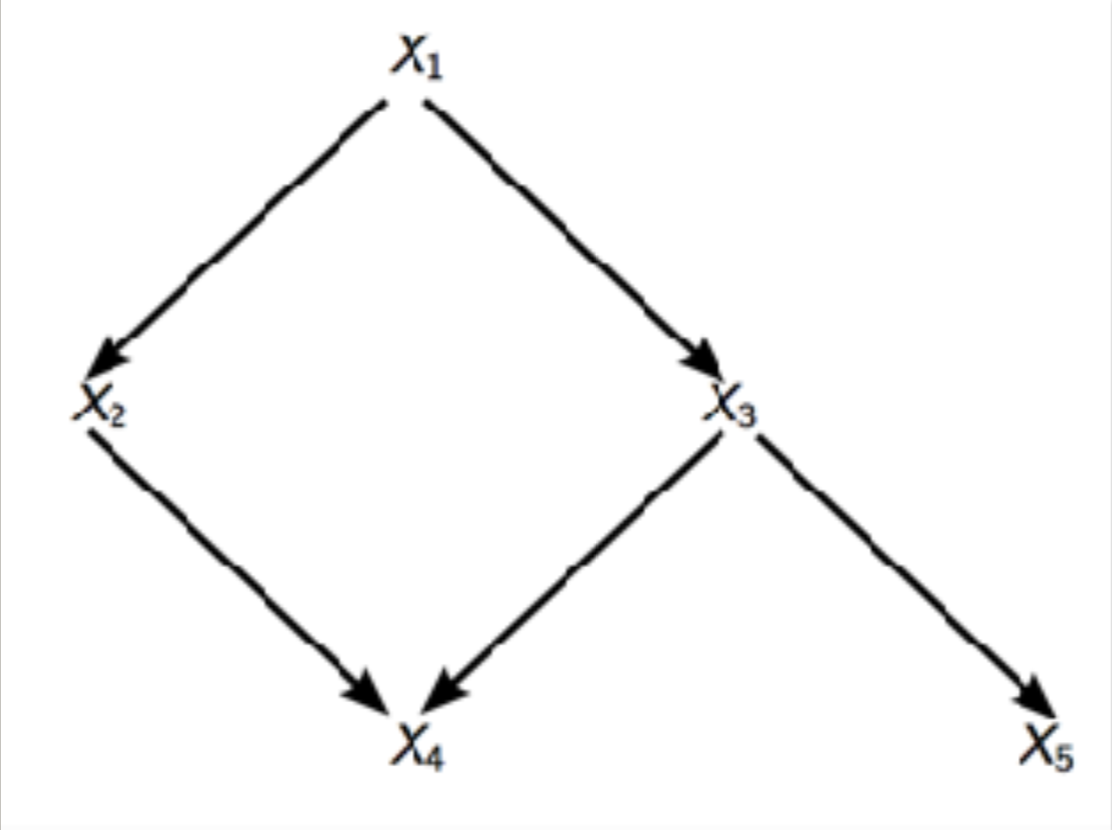
\includegraphics[scale=0.3]{images/bayesian-network-example.png}
    \caption{The example of Bayesian Network}
    \label{fig:my_label}
\end{figure}

\textit{PS: The graph not exist cycles since it is illegal for one thing dependent its self.}

\textbf{The Chain Rule}: 

\begin{multline}
    P(X_1, ..., X_n) \\
    = P(X_1) \frac{P(X_1, X_2)}{P(X_1)} \frac{P(X_1, X_2, X_3)}{P(X_1, X_2)} \dots \frac{P(X_1, ..., X_n)}{P(X_1, \dots, X_{n-1})} \\
    = P(X_1)P(X_2|X_1)\dots P(X_n|X_1, ..., X_{n-1}) = \prod^n_{n=1}P(X_i| \sqcap(X_i))
\end{multline}

\textbf{Possible Values}: Suppose that $X_1, X_2, \dots, X_n$ is a binary distribution, the total number of possible values is $\sum^n_{i=1}2^{|\sqcap(x_i)|}$, since $0 \leq |\sqcap(x_i)| \leq i-1$, we have

\begin{equation}
    (\sum^n_{i=1}2^0=n) \leq \sum^n_{i=1}2^{|\sqcap(x_i)|} \leq (\sum^n_{i=1}2^{i-1} = 2^n-1)
\end{equation}

which means the possible values satisfy $independent \leq Bayesian Network \leq fully dependent$.



\section{Information and Inference}

\subsection{Linear Knowledge}

A base knowledge can be represented by a set of linear equations on a probability measure $P$:

\begin{equation}
    K = \sum^{n_j}_{i=1}a_{i,j}P(A_{i,j}) = b_j: j = 1, \dots,m
\end{equation}

\textit{Example of Knowledge}: Supposing there are three sections, red(r), blue(b) and green(g). And our knowledge base is the probability of red is twice to probability of blue, $K = \{ P(r) = 2P(b)\}$.

\begin{itemize}
    \item Let denotes $P(r) = p_1, P(b) = p_2, P(g) = p_3$.
    \item From $K$ we have that $p_1 = 2p_2$ also we know hint $p_1 + p_2 + p_3 = 1 \rightarrow p_3 = 1 - 3p_2$
    \item The $V(K) \subseteq V$ corresponding to all probability distributions which satisfy $K$
    \item $V(K) = \{ <2p_2, p_2, 1-3p_2> : 0 \leq p_2 \leq \frac{1}{3} \}$
    \item Notice $p_2 \leq \frac{1}{3}$ since we require $3p_2 \leq 1$ and $2p_2 \leq 1$
\end{itemize}

\textit{Recall some basic maths}:

\begin{itemize}
    \item $\log_2{x} = \frac{\ln{x}}{\ln{2}}$, let $y = log_a{x} \Rightarrow a^y = x \Rightarrow ln{a^y} = ln{x} \Rightarrow y = \frac{\ln{x}}{\ln{a}}$
    \item $\frac{d\ln{x}}{dx} = \frac{1}{x}$
    \item $\frac{d(-x\log_2{x})}{dx} = \frac{ d(-x \frac{\ln{x}}{\ln{2}})}{dx} = -\frac{1}{\ln{2}} \frac{d(x\ln{x})}{dx} = -\frac{1}{\ln{2}}(\ln{x} + x\frac{1}{x}) = -\log_2{x} - \frac{1}{\ln{2}}$
\end{itemize}


\subsection{Information and Entropy}

\textbf{Shannon’s Entropy Measure}: Let $W = \{ w_1, ..., w_n\}$ and $P(w_i) = p_i$ then the information content of this distribution is

\begin{equation}
    H := -\sum^N_{i=1}{p_{i}log_2(p_i)}
\end{equation}

\begin{itemize}
    \item $H$ is minimal when $p_j = 1$ and for some $j \in \{ 1, ..., n\}$ and $p_i = 0$ for all $i \neq j$
    \item $H$ is maximal when $p_i = \frac{1}{n}$ for $i = \{1, \dots, n\}$
\end{itemize}

\textit{Proof Maximal Entropy}: Let $p_n = 1 - \sum^{n-1}_{i=1}p_i$ and $H = \sum^{n}_{i=1} - p_{i}log_2{p_i}$

$$\frac{dH}{dp_i} = \frac{d(-p_{i}log_{2}p_i)}{dp_i} + \frac{d(-p_{n}log_{2}p_n)}{dp_i} = -log_{2}p_i - \frac{1}{\ln2} + log_{2}(1 - \sum^{n-1}_{i=1}p_i) + \frac{1}{\ln2}$$
$$\frac{dH}{dp_i}  = -log_{2}p_i + log_{2}(1 - \sum^{n-1}_{i=1}p_i)$$
$$\frac{dH}{dp_i} = 0 \Rightarrow log_2{p_i} = log_2{1 - \sum^{n-1}_{i=1}p_i} \Rightarrow p_i = p_n$$
$$1 = \sum^{n}_{i=1}p_i \Rightarrow p_i = \frac{1}{n}$$


\textbf{Center of Mass}: Suppose we give every element of $V(K)$ equal probability, then we obtain the probability distribution

\begin{equation}
    \hat{p_i} = \frac{\int_{V(K)}p_{i}dV(K)}{\int_{V(K)}dV(K)}
\end{equation}

$<\hat{p_1}, \dots, \hat{p_n}>$ is the centre of mass of $V(K)$.

\textit{Example of CM}: For $V(K) = \{<p_1, 0.8-p_1, 0.7-p_1, p_1-0.5>: 0.5 \leq p_1 \leq 0.7\}$, 

$$\hat{p_1} = \int_{V(K)}p_{1}dV(K) = \frac{\int_{0.5}^{0.7}p_{1}dp_1}{\int_{0.5}^{0.7}dp_1} = \frac{0.12}{0.2} = 0.6$$



\section{Dempster-Shafer Theory}

\subsection{Mass Assignments}

Shafer-Dempster belief functions are defined by a probability distirbution on the power set of $W$.

\begin{equation}
    m: 2^w \rightarrow [0, 1], m(\varnothing) = 0, \sum_{A \subseteq W}{ m(A) = 1}
\end{equation}

\textbf{Belief and Plausibility}

\begin{itemize}
    \item Belief $Bel: 2^W \rightarrow [0, 1]$ is a measure of the total amount of evidence in favor of a proposition
    \begin{equation}
        Bel(A) = \sum_{B \subseteq A}{m(B)}
    \end{equation}
    \item Plausibility $Pl: 2^W \rightarrow [0, 1]$ is a measure of the total amount of evidence not against a proposition.
    \begin{equation}
        Pl(A) = \sum_{B: B\cap A \neq \varnothing}m(B)
    \end{equation}
    \item $\forall A \subseteq W$, $Bel(A) \leq Pl(A)$ and $Pl(A) - Bel(A)$ provides a direct measure of ignorance about the proposition $A$
    \item $Bel(A) + Bel(A^c) \leq 1$
    \item $Pl(A) = 1 - Bel(A^c)$
    \item Belief is sub-additive: $Bel(A \cup B) \geq Bel(A) + Bel(B)$
    $$Bel(A \cup B) = \sum_{C \subseteq A \cup B}{m(C)} = \sum_{C \subseteq A }{m(C)} + \sum_{C \subseteq B}{m(C)} + \sum_{C \subseteq A \cup B, C \nsubseteq A, C \nsubseteq B}{m(C)}$$
    $$\geq \sum_{C \subset A}{m(C)} + \sum_{C \subset B}{m(C)} = Bel(A) + Bel(B)$$
    \item Plausibility is super-additive: $Pl(A \cup B) \leq Pl(A) + Pl(B)$
    $$Pl(A \cup B) = \sum_{C \cap (A \cup B) \neq \varnothing}m(C) = \sum_{C \cap A \neq \varnothing}m(C) + \sum_{C \cap B \neq \varnothing}m(C) $$
    $$- \sum_{C \cap A \neq \varnothing, C \cap B \neq \varnothing}m(C) \leq \sum_{C \cap A \neq \varnothing}m(C) + \sum_{C \cap B \neq \varnothing}m(C) = Pl(A) + Pl(B)$$
\end{itemize}

\textbf{Belief Inversion}: If we already have the Belief and we want to know the Mass, we can consider different levels of each elements.

\begin{equation}
    m(A) = \sum_{B \subseteq A}(-1)^{|A - B|}Bel(B)
\end{equation}

\begin{equation}
    m(A) = \sum_{B \subseteq A}(-1)^{|A - B|}(1 - Pl(B^c))
\end{equation}

\textbf{Lower and Upper Probabilities}: A lower probability $\underline{P}: 2^W \rightarrow [0, 1]$ and an upper probability $\overline{P}: 2^W \rightarrow [0, 1]$
\begin{itemize}
    \item $\forall A \subseteq W\ \ \underline{P}(A) \leq \overline{P}(A)$
    \item $\forall A \subseteq W\ \ \overline{P}(A^c) = 1 - \underline{P}(A)$
\end{itemize}

$\mathbb{P}$ is a set of probability measures on $2^W$, then $\underline{P}(A) = inf \{ P(A): P \in \mathbb{P} \}$ and $\overline{P}(A) = sup\{ P(A): P \in \mathbb{P} \}$.


\subsection{Updating Probabilities}

Suppose we have a prior probability measure $P$ and evidence about the true state of the world is given by mass assignment $m$. To get a single probability measure we could then take the expected value:

\begin{equation}
    P( \bullet | m) = \sum_{B \subseteq W}P(\bullet | B)m(B) 
\end{equation}

\textit{Example for Updating Probabilities}:

$$P(w_1)=0.5,\ P(w_2)=0.3,\ P(w_3)=0.2$$
$$P(w_1 | \{w_1, w_2\}) = \frac{P(w_1)}{P(w_1) + P(w_2)} = \frac{5}{8}$$
$$P(w_2 | \{w_1, w_2\}) = \frac{P(w_2)}{P(w_1) + P(w_2)} = \frac{3}{8}$$
$$P(w_3 | \{w_1, w_2\}) = \frac{P(w_3)}{P(w_1) + P(w_2)} = 0 \ since\ \{w_3\} \cap \{w_1, w_2\} = \varnothing$$

\textbf{Pignistic Distribution}: Take  to be the uniform measure so that

\begin{equation}
    P_u(A | m) = \sum_{B \subseteq W}\frac{|A \cap B|}{|B|}m(B)
\end{equation}

where $|A|$ means the number of elements in set $A$.


\subsection{Nested Evidence}

\textbf{Nested hierarchy}: There exists $F_1 \subseteq F_2 \subseteq \dots \subseteq F_n \subseteq W$ such that $\sum^n_{i=1}m(F_i)=1$, $F_1 \subseteq F_2 \subseteq \dots \subseteq F_n \subseteq W$ are called the \textbf{focal sets} of $m$.

\textit{Example for Nested hierarchy}: There are $W=\{d_1, d_2, h\}$, suppose all doctors agree that the patient may have disease $d_2$, a subset of doctors think that he may have disease $d_1$, some doctors in this subset also believe it is possible that he is healthy.

\textbf{Possibility and Necessity Measures}: For a nested mass assignment the corresponding belief measure is called a \textbf{necessity measure} and the plausibility measure is called a \textbf{possibility measure}.

\begin{itemize}
    \item Let $F_j$ be the largest focal set for which $F_j \subseteq A$ then:
    \begin{equation}
        Bel(A) = Nec(A) = \sum_{B \subseteq A}m(B) = \sum^{j}_{i=1}m(F_i)
    \end{equation}
    \item Let $F_k$ be the smallest focal set for which $A \cap F_k \neq \varnothing$ then:
    \begin{equation}
        Pl(A) = Pos(A) = \sum_{B:B \cap A \neq \varnothing}m(B) = \sum^{n}_{i=k}m(F_k)
    \end{equation}
\end{itemize}

\textbf{Possibility and Necessity Axioms}

\begin{itemize}
    \item \textbf{Pos1}: $Pos(W) = 1, Pos(\varnothing)=0$
    \item \textbf{Pos2}: $Pos(A \cup B) = max(Pos(A), Pos(B))$
    \item \textbf{Nec1}: $Nec(W) = 1, Nec(\varnothing)=0$
    \item \textbf{Nec2}: $Nec(A \cap B) = min(Nec(A), Nec(B))$
    \item \textbf{Consequences1}: $\forall A \subseteq W$, $Pos(A) = 1$ or $ Pos(A^c) = 1$. Notice that $$1 = Pos(W) = Pos(A \cup A^c) = max(Pos(A), Pos(A^c))$$
    \item \textbf{Consequences2}: $\forall A \subseteq W$, $Nec(A) = 0$ or $Nec(A^c) = 0$. Notice that $$0 = Nec(\varnothing) = Nec(A \cap A^c) = min(Nec(A), Nec(A^c))$$
    \item Either $[Nec(A), Pos(A)] = [x, 1]$ or $[0, y]$ where $0 < x \leq 1$ and $0 \leq y < 1$.
\end{itemize}

\textit{Proof if $Nec(A) > 0$ then $Pos(A) = 1$}: 

\begin{itemize}
    \item $Pos(A^c) = 1 - Nec(A)$ therefore $Nec(A) > 0 \Rightarrow Pos(A^c) < 1$. 
    \item Now $1 = Pos(W) = Pos(A \cup A^c) = max(Pos(A), Pos(A^c))$.
    \item Hence, since $Pos(A^c) < 1$ so that $Pos(A) = 1$.
\end{itemize}

\textbf{Possibility Distribution}: For any $A \subseteq W$, $Pos(A) = max\{ Pos(\{w_i\}): w_i \in A \}$. Let $Pos(\{w_i\}) = \pi(w_i)$ and $max \{ \pi(w_i): w_i \in W \} = 1$.

\textbf{Possibility Inversion}: Suppose $W = \{ w_1, \dots, w_n\}$ ordered, then

$$1 = \pi(w_1) \geq \pi(w_2) \geq \dots \geq \pi(w_n)$$
$$m(\{w_1, \dots, w_n \}) = \pi(w_n)$$
$$m(\{w_1, \dots, w_{n-1} \}) = \pi(w_{n-1}) - \pi(w_n)$$
$$m(\{w_1, \dots, w_i \}) = \pi(w_i) - \pi(w_{i+1}) $$
$$m(\{w_1\}) = 1 - \pi(w_2)$$


\subsection{Demspter’s Rule of Combination}

Suppose we have two mass assignments provided by two independent sources of evidence.

\begin{equation}
    \forall A \subseteq W\ \ m_1 \bigoplus m_2 (A) = \frac{\sum_{(B, C: B \cap C = A)} m_1(B)m_2(C)}{1 - \sum_{(B, C): B \cap C = \varnothing}m_1(B)m_2(C)}
\end{equation}

\textbf{Conditional Belief Functions}: Suppose that $Pl$ is a plausibility:

\begin{equation}
    Pl(A | B) = \sum_{C \subseteq W; C \cap A \neq \varnothing} m \bigoplus m_B(C) = \frac{Pl(A \cap B)}{Pl(B)}
\end{equation}

Notice that $m \bigoplus m_B(C) = \frac{\sum_{C: C \cap A \neq \varnothing}m(D)}{1-\sum_{D:D\cap B = \varnothing}m(D)}$

$$Pl(A | B) = \frac{\sum_{D:(D \cap B) \cap A \neq \varnothing} m(D)}{1 - \sum_{D: D \cap B = \varnothing}m(D)}=\frac{\sum_{D:(D\cap B)\cap A \neq \varnothing}m(D)}{\sum_{D:D\cap B \neq \varnothing}m(D)} = \frac{Pl(A\cap B)}{Pl(B)}$$

Also 

\begin{multline}
    Bel(A | B) = 1 - Pl(A^c | B) = 1 - \frac{Pl(A^c \cap B)}{Pl(B)} = \frac{Pl(B) - Pl(A^c \cap B)}{Pl(B)} = \\ \frac{(1 - Bel(B^c)) - (1 - Bel(A \cup B^c))}{1 - Bel(B^c)} = \frac{Bel(A \cup B^c) - Bel(B^c)}{1 - Bel(B^c)}
\end{multline}



\section{Fuzzy Set Theory}

Fuzzy sets are sets to which elements can belong to some partial degree. A (crisp) set $A \subseteq W$ can be characterised by a membership function $\chi_A: W \rightarrow \{0, 1\}$ so that 

\begin{equation}
    \chi_A = \left\{\begin{matrix} 1: & w \in A \\  0: & w \notin  A \end{matrix}\right.
\end{equation}


The support of a fuzzy set $\tilde{A}$ is given by $Sup(\tilde{A}) = \{ w \in W: \chi_{\tilde{A}}(w)>0 \}$ and the fuzzy set is

\begin{equation}
    \tilde{A} = \sum_{w \in Supp(\tilde{A})} w / \chi_{\tilde{A}} (w)
\end{equation}

\textbf{Sorites Paradox}: Consider a man with a lot of hair on his head. One hair is plucked at a time until he is bald. It follows that there must be a hair pluck at which the man switches from being not bald to being bald. However, this is counter intuitive since the difference of one hair cannot induce a category change from not bald to bald. This or an alternative version of sorites.


\subsection{T-norm}

\textbf{T-norm} are function $T: [0, 1]^2 \rightarrow [0, 1]$ which satisfy the following properties:

\begin{itemize}
    \item \textbf{T1}: $\forall x \in [0, 1]\ \ T(x, 1) = x$
    \item \textbf{T2}: $\forall x, y, z \in [0, 1]$, if $y \leq z$ then $T(x, y) \leq T(x, z)$
    \item \textbf{T3}: $\forall x, y \in [0, 1], T(x, y) = T(y, x)$
    \item \textbf{T4}: $\forall x, y, z \in [0, 1], T(x, T(y, z)) = T(T(x, y), z)$
    $$\varphi_{(A \cap B) \cap C} = \varphi_{A \cap (B \cap C)} \Rightarrow T(T(A, B), C) = T(A, T(B, C))$$
    \item \textbf{T5}: $\forall x \in [0, 1]$ $T(x, x) = x$
\end{itemize}

\textbf{Theorem}: For any t-norm $T$, $drastic \leq T \leq min$, where 

\begin{equation}
    drastic(x, y) = \left\{\begin{matrix} x & : & y = 1\\ y & : & x = 1\\ 0 & : & otherwise \end{matrix}\right.
\end{equation}

\begin{itemize}
    \item Show that $T \leq min(x, y)$
    $$T(x, y) \leq T(x, 1) = x$$
    $$T(x, y) = T(y, x) \leq T(y, 1) = y $$
    $$T(x, y) \leq min(x, y)$$
    \item Show that $T \geq drastic(x, y)$
    $$T(x, 1) = x$$
    $$T(1, y) = T(y, 1) = y$$
    $$T(x, y) \geq 0$$
    $$T(x, y) \geq drastic$$
\end{itemize}

\textbf{Families of T-norms}

\begin{itemize}
    \item \textbf{Frank’s t-norms}: $T_s(x, y) = log_s[1 + \frac{(s^x-1)(s^y-1)}{s-1}]$ where $s > 0$ and $s \neq 1$
    \item \textbf{Dombi Family}: $T_{\lambda}(x, y) = \{ 1 + [(\frac{1}{x} - 1)^{\lambda} + (\frac{1}{y} - 1)^{\lambda}]^{\frac{1}{\lambda}} \}^{-1}$, where $\lambda > 0$
\end{itemize}


\subsection{T-conorms}

\textbf{T-conorms} are function $S: [0, 1]^2 \rightarrow [0, 1]$, it equal to $1 - T(1-x, 1-y)$ and satisfy the following properties:

\begin{itemize}
    \item \textbf{S1}: $\forall x \in [0, 1]$ $S(x, 0) = x$
    \item \textbf{S2}: $\forall x, y, z \in [0, 1]$ if $y \leq z$ then $S(x, y) \leq S(x, z)$
    \item \textbf{S3}: $\forall x, y \in [0, 1]$ $S(x, y) = S(y, x)$
    \item \textbf{S4}: $\forall x, y, z \in [0, 1]$ $S(x, S(y, z)) = S(S(x, y), z)$
    \item \textbf{S5}: $\forall x \in [0, 1]$ $S(x, x) = x$
\end{itemize}


\subsection{Fuzzy Set}

\textbf{$\alpha$-cuts} provide a way of representing fuzzy sets as a nested sequence of crisp sets, Fuzzy set $\tilde{A}_{\alpha} = \{ w \in W: \chi_{\tilde{A}}(w) \geq \alpha \}$ so $\chi_{\tilde{A}}(w) = \int_{\alpha:w\in\tilde{A}_{\alpha}}d\alpha$.

Notice that $w \in \tilde{A}_{\alpha}$ if and only if $\varphi_{\tilde{A}}(w) \geq \alpha$, therefore $\{ \alpha: w \in \tilde{A}_{\alpha} \} = (0, \chi_{\tilde{A}}(w)]$.

\textit{Example for Fuzzy Set}: There are $\tilde{A} = 5/1 + 6/0.8 + 7/05$ and $\tilde{B} = 1/1+ 2/0.5 + 3/0.2$, use the $\alpha$-cut method to determine $\frac{\tilde{A}}{\tilde{B}}$.

\begin{table}[h]
    \centering
    \begin{tabular}{|c||c|c|c|}
        \hline
        $\frac{\tilde{A}}{\tilde{B}}$ & $\{5, 6, 7\}:(0, 0.5]$ & $\{5, 6\}:(0.5, 0.8]$ & $\{5\}:(0.8, 1]$\\
        \hline
        \hline
        $\{1, 2, 3\}:(0, 0.2]$ & $\{5,6,7,\frac{5}{2},3,\frac{7}{2},\frac{5}{3},2,\frac{7}{3}\}:(0,0.2]$ & $\varnothing$ & $\varnothing$ \\
        \hline
        $\{1, 2\}:(0.2, 0.5]$ & $\{5,6,7,\frac{5}{2},3,\frac{7}{2}:(0.2,0.5]$ & $\varnothing$ & $\varnothing$ \\
        \hline
        $\{1\}:(0.5, 1]$ & $\varnothing$ & $\{5,6\}:(0.5,0.8]$ & $\{5\}:(0.8,1]$ \\
        \hline
    \end{tabular}
    \label{tab:my_label}
\end{table}

$$\tilde{A}_{\alpha} = \left\{\begin{matrix} \{5, 6, 7\} & : & \alpha \in (0, 0.5] \\  \{5, 6 \}  & : & \alpha \in (0.5, 0.8] \\ \{5 \} & : & \alpha \in (0.8, 1] \end{matrix}\right.\ and\ \tilde{B}_{\alpha} = \left\{\begin{matrix} \{1, 2, 3\} & : & \alpha \in (0, 0.2] \\  \{1, 2 \}  & : & \alpha \in (0.2, 0.5] \\  \{1 \} & : & \alpha \in (0.5, 1] \end{matrix}\right. $$



$$(\frac{\tilde{A}}{\tilde{B}})_{\alpha} = \left\{\begin{matrix} \{5,6,7,\frac{5}{2},3,\frac{7}{2},\frac{5}{3},2,\frac{7}{3}\} & : & \alpha \in (0,0.2] \\  \{5,6,7,\frac{5}{2},3,\frac{7}{2} & : & \alpha \in (0.2,0.5] \\ \{5,6\} & : & \alpha \in (0.5,0.8] \\ \{5\} & : & \alpha \in (0.8,1] \end{matrix}\right.$$

$$\frac{\tilde{A}}{\tilde{B}} = 5/1 + 6/0.8 + 7/0.5 + \frac{5}{2}/0.5 + 3/0.5 + \frac{7}{2}/0.5 + 5/0.2 + 6/0.2 + 7/0.2$$



\section{Model Logic}

The idea is to directly incorporate the notions of possibly the case and necessarily the case directly in to a formal logic.

\textbf{Proposition}: $w \models A$ denote that proposition $A$ is true in world $w$.

\begin{equation}
    W(A) = \{ w \in W: w \models A \}
\end{equation}

\textbf{Well-Formed Formula}

\begin{itemize}
    \item standard connectives: $\neg$ (not), $\wedge$ (and), $\vee$ (or)
    \item modal operators: $\square$ (necessarily), $\diamond$ (possibly)
    \begin{itemize}
        \item $\square \theta$ means $\theta$ is necessarily the case.
        \item $\diamond \theta$ means $\theta$ is possibly the case.
    \end{itemize}
\end{itemize}


\textbf{Semantics of  Modal Logic}

\begin{itemize}
    \item $w \models \square \theta$: for all $w'$ such that $Edge(w, w'), w' \models \theta$
    \item $w \models \diamond \theta$: if $\theta$ is true in every world accessible from $w$, there exists $w'$ such that $Edge(w, w'), w' \models \theta$
    \item $W(\square B) \subseteq W(B) \subseteq W( \diamond B)$
    \item $\theta \models \varphi$ ($\theta$ entails $\varphi$ or $\varphi$ follows $\theta$) if and only if $w \models \theta$ implies that $w \models \varphi$
    \item $\neg \square \neg \theta \equiv \diamond \theta$ and $\neg \diamond \neg \theta \equiv \square \theta$
\end{itemize}

\textbf{Properties of Relations}

\begin{itemize}
    \item Reflexive: $E(w, w)$ for all $w \in W$
    \item Symmetric: If $E(w, w')$ then $E(w', w)$
    \item Transitive: If $E(w_1, w_2)$ and $E(w_2, w_3)$ then $E(w_1, w_3)$
    \item Dense: If $E(w_1, w_3)$ then there exists $w_2$ such that $E(w_1, w_2)$ and $E(w_2, w_3)$
    \item Serial: For all $w$, there exists $w'$ such that $E(w, w')$
    \item Identity Relation: $E(w, w')$ if and only if $w = w'$
\end{itemize}

\textbf{Probability, Model Logic and DS-Theory}: $P$ is a probability measure on $2^W$; $R(w)$ is the set of worlds which are reachable from $w$ denoted as $R(w) = \{ w' : E(w, w') \}$. Notice that $w \models \theta$ if and only if $R(w) \subseteq W(\theta)$, $w \models \diamond \theta$ if and only if $R(w) \cap W(\theta) \neq \varnothing$.

Mass function: $m(F) = P(\{ w: R(w) = F \}) = \sum_{w:R(w)=F}P(w)$

If $E$ is serial then for all $w$, $R(w) \neq \varnothing$ and hence $m(\varnothing) = 0$, $P(\square \theta) = Bel(\theta)$ and $P(\diamond\theta) = Pl(\theta)$.

$$P(\square \theta) = P(W(\square \theta)) = \sum_{w: R(w)\subseteq W(\theta)}P(w)$$
$$= \sum_{F \subseteq W(\theta)}\sum_{w:R(w)=F}P(w) = \sum_{F\subseteq W(\theta)}m(F) = Bel(W(\theta)) = Bel(\theta)$$

and also $P(\diamond \theta) = P(\neg \square \neg \theta)  = 1- P(\square \neg \theta) = 1 - Bel(\neg \theta) = Pl(\theta)$.


\textit{Web page Example}: Consider the probability distribution $\{ w_1, w_2, w_3, w_4, w_5 \}$

\begin{figure}[h]
    \centering
    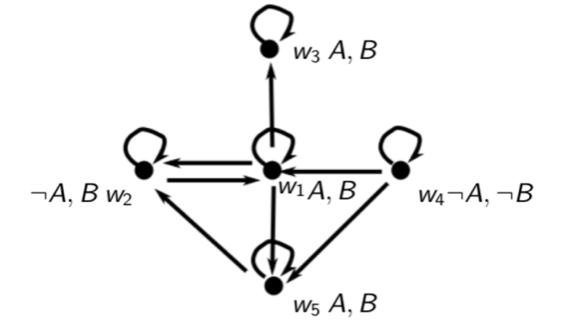
\includegraphics[scale=1]{images/example-web-page.png}
    \caption{Web Page}
    \label{fig:my_label}
\end{figure}


$$P(w_1) = 0.1, P(w_2) = 0.2, P(w_3) = 0.2, P(w_4) = 0.4, P(w_5) = 0.1$$
$$R(w_1) = \{w_1, w_2, w_3, w_5\}, R(w_2) = \{ w_1, w_2 \}, R(w_3) = \{ w_3 \}$$
$$R(w_4) = \{w_1, w_4, w_5 \}, R(w_5) = \{ w_2, w_5 \}$$
$$W(B) = \{w_1, w_2, w_3, w_5 \}$$
$$Bel(B) = m(\{w_1, w_2, w_3, w_5 \}) + m(\{ w_1, w_2 \}) + m(\{ w_3 \}) + m(\{ w_2, w_5 \}) = 0.6$$
\end{document}
